\documentclass[10pt,final,a4paper,oneside,onecolumn]{article}

%%==========================================================================
%% Packages
%%==========================================================================
\usepackage[a4paper,left=3.5cm,right=3.5cm,top=3cm,bottom=3cm]{geometry} %% change page layout; remove for IEEE paper format
\usepackage[T1]{fontenc}                        %% output font encoding for international characters (e.g., accented)
\usepackage[cmex10]{amsmath}                    %% math typesetting; consider using the [cmex10] option
\usepackage{amssymb}                            %% special (symbol) fonts for math typesetting
\usepackage{amsthm}                             %% theorem styles
\usepackage{dsfont}                             %% double stroke roman fonts: the real numbers R: $\mathds{R}$
\usepackage{mathrsfs}                           %% formal script fonts: the Laplace transform L: $\mathscr{L}$
\usepackage[pdftex]{graphicx}                   %% graphics control; use dvips for TeXify; use pdftex for PDFTeXify
\usepackage{array}                              %% array functionality (array, tabular)
\usepackage{upgreek}                            %% upright Greek letters; add the prefix 'up', e.g. \upphi
\usepackage{stfloats}                           %% improved handling of floats
\usepackage{multirow}                           %% cells spanning multiple rows in tables
%\usepackage{subfigure}                         %% subfigures and corresponding captions (for use with IEEEconf.cls)
\usepackage{subfig}                             %% subfigures (IEEEtran.cls: set caption=false)
\usepackage{fancyhdr}                           %% page headers and footers
\usepackage[official,left]{eurosym}             %% the euro symbol; command: \euro
\usepackage{appendix}                           %% appendix layout
\usepackage{xspace}                             %% add space after macro depending on context
\usepackage{verbatim}                           %% provides the comment environment
\usepackage[dutch,USenglish]{babel}             %% language support
\usepackage{wrapfig}                            %% wrapping text around figures
\usepackage{longtable}                          %% tables spanning multiple pages
\usepackage{pgfplots}                           %% support for TikZ figures (Matlab/Python)
\pgfplotsset{compat=1.14}						%% Run in backwards compatibility mode
\usepackage[breaklinks=true,hidelinks,          %% implement hyperlinks (dvips yields minor problems with breaklinks;
bookmarksnumbered=true]{hyperref}   %% IEEEtran: set bookmarks=false)
%\usepackage[hyphenbreaks]{breakurl}            %% allow line breaks in URLs (don't use with PDFTeX)
\usepackage[final]{pdfpages}                    %% Include other pdfs
\usepackage[capitalize]{cleveref}				%% Referensing to figures, equations, etc.
\usepackage{units}								%% Appropriate behavior of units
\usepackage[utf8]{inputenc}   				 	%% utf8 support (required for biblatex)
\usepackage{csquotes}							%% Quoted texts are typeset according to rules of main language
\usepackage[style=ieee,doi=false,isbn=false,url=false,date=year,minbibnames=15,maxbibnames=15,backend=biber]{biblatex}
%\renewcommand*{\bibfont}{\footnotesize}		%% Use this for papers
\setlength{\biblabelsep}{\labelsep}
\bibliography{../../bib}

\newtheorem*{remark*}{Remark}

%%==========================================================================
%% Define reference stuff
%%==========================================================================
\crefname{figure}{Figure}{Figures}
\crefname{equation}{}{}

%%==========================================================================
%% Define header/title stuff
%%==========================================================================
\newcommand{\progressreportnumber}{33}
\renewcommand{\author}{Erwin de Gelder}
\renewcommand{\date}{August 12, 2020}
\renewcommand{\title}{Performance assessment of automated vehicles using real-world driving scenarios}

%%==========================================================================
%% Fancy headers and footers
%%==========================================================================
\pagestyle{fancy}                                       %% set page style
\fancyhf{}                                              %% clear all header & footer fields
\fancyhead[L]{Progress report \progressreportnumber}    %% define headers (LE: left field/even pages, etc.)
\fancyhead[R]{\author, \date}                           %% similar
\fancyfoot[C]{\thepage}                                 %% define footer

\begin{document}
	
\begin{center}
	\begin{tabular}{c}
		\title \\ \\
		\textbf{\huge Progress report \progressreportnumber} \\ \\
		\author \\ 
		\date
	\end{tabular}
\end{center}

\section{Previous meeting minutes}

\begin{itemize}
	\item We discussed the method I used for the scenario risk quantification. The only comments was that for the case study, it might be enough to compare a human driver with an fully automated vehicle, such that I do not need to model a human interacting with an automated vehicle.
	\item We discussed my plans for revising the rejected paper \textit{ontology for scenarios for the assessment of automated vehicles}. 
\end{itemize}

\section{Summary of work}

\begin{itemize}
	\item I revised the paper \textit{ontology for scenarios for the assessment of automated vehicles}, now titled: \textit{Scenarios for the Assessment of Automated Vehicles: An Object-Oriented Framework}. The revised paper is attached to this report (starting at page 5). The changes are marked by a gray bar and red font.
	
	\item I started with writing of the paper \textit{Scenario Risk Quantification for Automated Driving}. The current draft is attached to this report (starting at page 35).
\end{itemize}

\section{Future plans}

In \cref{fig:planning}, the updated planning is shown. The following list contains the articles I want to write for my PhD. I also listed articles that I think are too ambitious to write, but I added them nevertheless so that we can discuss them if needed.
\begin{itemize}
	\item \textit{Ontology 1}: This is the article that has been rejected for publication in Transportation Research Part C: Emerging Technologies. There is already a version available on arXiv \cite{degelder2020ontology}. Nevertheless, I would like to publish the article to a journal to increase its visibility. In response to the criticism, I want to remove the word ``ontology'' and use ``object-oriented'' instead. The main reason is that the ontology is used to obtain an object-oriented framework, while an ontology could be used for more things (like reasoning). I foresee the following workload to rework this paper to a new version that can be submitted (8 days in total):
	\begin{itemize}
		\item Update the paper (2 days): Substitute ``object-oriented framework'' for ``ontology'' and do some rephrasing.
		\item Feedback (1 day): Collect and process feedback from the 8 (!) co-authors.
		\item Domain model update (2 days): The code is online available and needs few updates.
		\item Github tutorial (3 days): The main criticism was that the reviewer missed how the code could be of use. Therefore, I want to provide a tutorial explaining how the code can be effectively used to process and generate scenarios.
	\end{itemize}
	As a potential journal, I am thinking of \textit{IEEE Access}.
	
	\begin{figure}[t]
		\centering
		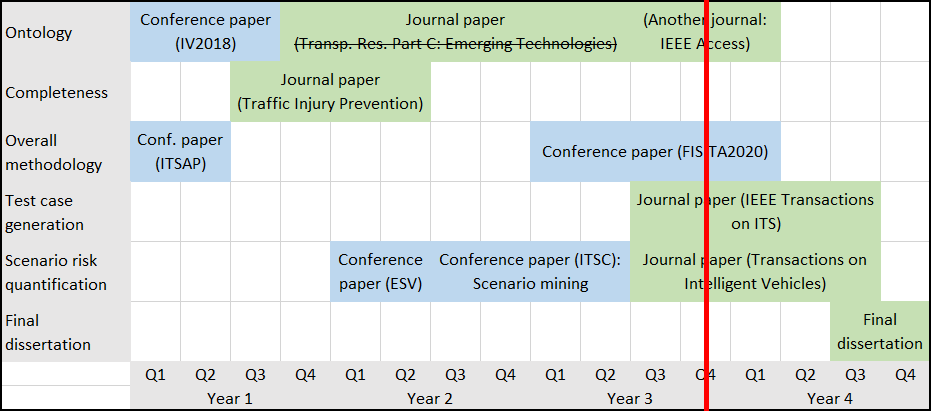
\includegraphics[width=\linewidth]{planning.png}
		\caption{Proposed planning at the time of this report. The red line indicated the time when writing this report.}
		\label{fig:planning}
	\end{figure}
	
	\item \textit{Ontology 2 (out-of-scope for PhD):} In this article, I want to use the ontology for reasoning. This can be a powerful tool when analyzing recorded microscopic traffic data. It can be used to enable a computer to infer that the following two scenario descriptions, which do not say the same thing, actually mean the same thing \cite{OpenSCENARIO2}:
	\begin{enumerate}
		\item A motorcycle cuts off an ADS truck, causing it to brake suddenly, and then a car that is behind the truck crashes into the side of the road.
		\item An ADS truck is driving in front of a car that crashes into the side of the road because the truck braked suddenly in response to a motorcycle that suddenly cut it off.
	\end{enumerate}
	I estimate the total work load to be at least 32 days:
	\begin{itemize}
		\item Build the ontology in Prot{\'e}g{\'e} (5 days)
		\item Perform a case study (5 days)
		\item Rewriting (15 days): Although parts can be re-used, we need to write a ``new'' paper.
		\item Review draft (3 days)
		\item Github update (2 days): I also want this to be available for the community.
		\item Revision (2 days)
	\end{itemize}

	\item \textit{Test case generation 1:} The main goal of this article is to present a method for generating realistic test cases that follow the same distribution as the recorded scenarios in the data set that is used. Here, the challenge is to deal with the large number of (correlated) parameters. My goal is to have a ``PowerPoint-version'' finished near the end of 2020. I estimate the total workload for this paper to be 33 days:
	\begin{itemize}
		\item Generalize the current method (5 days): I have a working version for the scenario category ``cut-in''. This method should be generalized such that it can be applied to any scenario category.
		\item Generalize the corresponding code (5 days)
		\item Provide two examples (2 days)
		\item Write article (15 days): method (5 days), case studies (5 days), introduction, background, and conclusion (5 days)
		\item Revision of draft (3 days)
		\item Submit and revise (3 days)
	\end{itemize}
	
	\item \textit{Test case generation 2 (out-of-scope for PhD):} Scenario-based testing is only useful for the safety assessment of automated vehicles (AVs) if the test cases focus on the critical scenarios. Because the statistical information is used to generate the test cases in the above article, it can be used to focus on the scenario that are critical and realistic. In this follow-up paper, I want to describe one such method that can be used to automatically focus on the more critical test cases. I estimate the total workload for this paper to be 41 days:
	\begin{itemize}
		\item Simplified AV model (2 days): We can only determine if something is critical if we know the system.
		\item Set up the simulator for the case study (3 days): Use can be made of existing work.
		\item Work out the method (5 days)
		\item Provide two examples (10 days)
		\item Write article (15 days): method (5 days), case studies (5 days), introduction, background, and conclusion (5 days)
		\item Revision of draft (3 days)
		\item Submit and revise (3 days)
	\end{itemize}
	
	\item \textit{Scenario risk quantification:} In this article, I want to present a method for estimating the 
	\begin{enumerate}
		\item exposure (through scenario mining in real-world data),
		\item severity (through simulations and literature), and
		\item controllability (through simulations).
	\end{enumerate}
	The main idea is already presented as the ESV conference \cite{degelder2019risk}. The method on estimating the exposure is already presented in our ITSC2020 paper \cite{degelder2020scenariomining}. The remaining work is to work out the case studies and to write the article. The goal is to submit a manuscript near the end of 2020. I estimate the total workload to be 34 days in total:
	\begin{itemize}
		\item Model the human-ADS interaction (3 days): This is almost done. 
		\item Perform the case studies (10 days): This is partly (50\%) done.
		\item Write  article (15 days): method (5 days), case studies (5 days), introduction, background, and conclusion (5 days)
		\item Revision of draft (3 days)
		\item Submit and revise (3 days)
	\end{itemize}
	
	\item \textit{Final dissertation:} The final dissertation is a collection of the written article with, in addition, a introduction and conclusions. I also want to ensure that the notation and terminology across the different articles is consistent. 
	
	I estimate that I will need 5 days for each of the five topics mentioned in \cref{fig:planning} and another 20 days for the introduction and conclusions and finalizing the dissertation. So a total of 45 days of workload is anticipated.
\end{itemize}

Considering the three articles that I want to write (\textit{ontology 1}, \textit{test case generation 1}, and \textit{scenario risk quantification}), I need 75 days. Assuming that I can work 2.5 days per week on my PhD, this will take 30 weeks. Considering my holidays, this should be finished in Q2 of 2021, so that I have 3 to 4 months left for my dissertation. 

\begin{remark*}
	This is if everything goes according to plan. Knowing myself, I might be a bit too optimistic regarding the real time I need. However, I still hope that I can finish everything before the end of 2021.
\end{remark*}

\section{Questions}

\begin{itemize}
	\item Regarding the planning:
	\begin{itemize}
		\item Is it feasible?
		\item Do I focus on the right things?
		\item If I succeed with my plans, will it be sufficient for my PhD?
	\end{itemize}

	\item Regarding the paper ``Scenarios for the Assessment of Automated Vehicles: An Object-Oriented Framework'':
	\begin{itemize}
		\item Would \textit{IEEE Access} be a suitable journal? When looking for similar papers in the field of \emph{Intelligent Transportation Systems}, I only found \textit{Transportation Research Part C: Emerging Technologies} and \textit{IET Intelligent Transport Systems} to have similar type of articles. Because this article got rejected for the former journal and the latter journal seems very low quality, I though of \textit{IEEE Access}. \textit{IEEE Access} seems to be a broad journal that has at least one very interesting paper related to the same topic \cite{riedmaier2020survey}.
	\end{itemize}
	\item Regarding the paper ``scenario risk quantification for automated driving'':
	\begin{itemize}
		\item For estimating the exposure, the method described in our ITSC2020 paper is used \cite{degelder2020scenariomining}. I wonder to what extent we need to explain the method presented in \cite{degelder2020scenariomining} in the current paper. Explaining the whole method would lead to another 10 pages, so that seems a bit too much. Since the method in \cite{degelder2020scenariomining} consists of two parts, I am thinking of only presenting the second part. 
	\end{itemize}
\end{itemize}


\printbibliography

\clearpage
\includepdf[pages=-,pagecommand={},width=\paperwidth]{../../"20180629 Journal paper ontology"/framework_scenarios.pdf}
\includepdf[pages=-,pagecommand={},width=\paperwidth]{../../"20191113 Journal Scenario Risk"/scenario_risk.pdf}

\end{document}